
\paragraph{Community Engagement}
Climate events are occurring with increasing rapidity. 
Our effort hopes to break ground with demonstration cases that spur partnerships across public and private sectors, span government agencies, and cross the divide between cultural and socioeconomic groups.
Such partnerships are a requisite element \cite{SDGs} that underlies any national effort to build adaptive and resilient energy and climate strategies and policies that can leverage the latest emerging technologies in AI, machine learning, robotics, and applied mathematics. 
This initiative will lead the path for robust and adaptive precision agriculture and an intelligent equitable energy strategy that at once recognizes the individual interests of all active participants and shareholders, while predicting climate and humanitarian events, and optimizing dynamic adaptation to accommodate and even capitalize on them.
Initiated under the auspices of an open-source community group called The Enterprise Neurosystem which includes members from SLAC/Stanford, multiple universities, and private and public companies, our community is coalescing around a very wide-reaching effort for an AI infrastructure that promotes climate resilience via adaptive agricultural practices, and provides course correction recommendations that mitigate the human and environmental impact of climate events.
As an initial demonstration of the utility of broad information sharing for model training, the team is working in close collaboration with the Department of Energy's Artificial Intelligence and Technology Office (AITO) to develop the secure integration of distributed datasets that intentionally span multiple scientific domains. 
This can be achieved with a federation model that preserves data privacy as needed, openly exposes publicly shared data where available, and creates mutually beneficial AI models that generalize across domains of human knowledge.

\paragraph{The Hive Mind}
Our pursuit of active adaptation to climate events will foster resilient agriculture and energy systems with the aim to bring artificial intelligence centrally into the task of integrating the full range of human environmental monitoring and response. 
We have an ultimate goal of overlaying climate-relevant satellite imagery with local agricultural health.
We have begun with a project developed from a grass-roots partnership between the DOE's AITO, SLAC's cross-domain EdgeAI research, and the open-source community of industry partners--the Enterprise Neurosystem.
Our shared vision is to merge together information from multiple modes of environmental monitoring and at vastly different geospatial scales.

\begin{wrapfigure}{l}{.5\linewidth}
	\centerline{
		\includegraphics[trim={0 150 0 50},clip,width=\linewidth]{./localfigs/Composite.jpg}
		}
		\vspace{-1\baselineskip}
	\caption{\label{fig::composite}
		Composite of satellite imaging of various modalities, and regions, based on Refs.~\cite{YaraGlaciers,TomasBeaches,GlobalCO2,SurfaceWater} for a-d respectively.
		}
\end{wrapfigure}

For instance, global scale environmental satellite imagery (Fig.~\ref{fig::composite}), from meters to kilometers, can provide a family of diagnostic overlays for point samples on the ground, or in the water as shown in Fig.~\ref{fig::composite}d adapted from Ref.~\cite{SurfaceWater}.
Such overlays individually focus in on, e.g., crop diversity and regional pollution from refuse \cite{TomasBeaches}, agricultural runoff \cite{NeonicsOnBees} as well as aquifer \cite{GRACE_CongoBasinWatershed} and glacier health \cite{YaraGlaciers}, and surface water concentrations \cite{SurfaceWater}. 
And while a satellite modality might capture CO$_2$ concentration \cite{GlobalCO2} at the kilometer meter scale, urban and agricultural beehive health could give a finer mesh of overall environmental health.

Correlating hive health with variations in numerous environmental factors is just the job of data-hungry machine learning algorithms. 
But this project starts with a few beehives at a time. 
Given the wealth of large-scale satellite imagery available, we have turned our attention to ground-level primary sources, thus we plan to ask the bees themselves.

Stanford collaborator Dr. Tadashi Fukami uses precise individual bee microbiome analysis \cite{Fukami2022} to reconstruct the nectar diversity for a hive. 
One can imagine point measurements of nectar diversity attributing spatial labels into geospatial images much like the water sample points (dots) in Fig.~\ref{fig::composite}d.
Our team is currently focused on continuous passive acoustic monitoring that would add point measurements of hive health and state. 
Starting small and local, we are quickly growing to partner with a much broader diversity of hive locations across complementary environments--industrial and local agricultural sites, native tribal lands, urban sites, and international sites where domestication of native honeybee species is a common practice.

Growth into diverse environments is precisely the benefit of engaging with the AITO.
By working directly with typically under-engaged institutions that represent the agricultural and urban demographics that are key to project success, AITO is helping foster AI development in the communities that will likely have an outsized positive impact on the future of climate adaptability.

\begin{figure}
	\centerline{a.\hspace{.5\linewidth}b.}
	\centerline{
		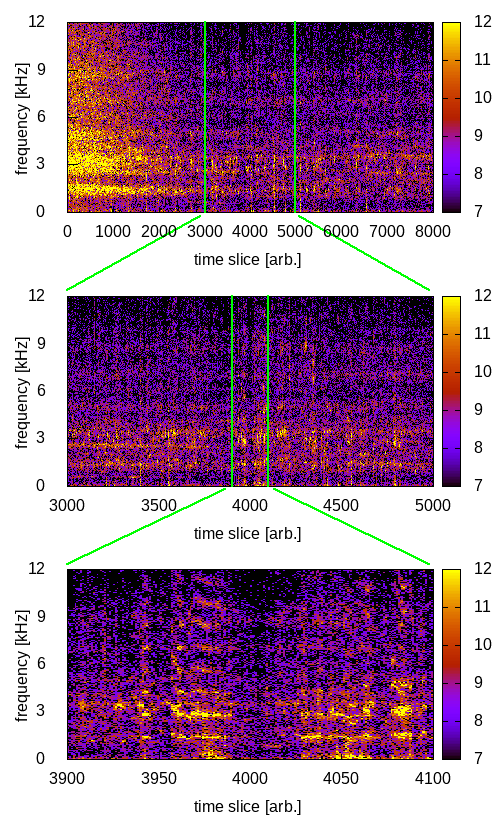
\includegraphics[clip,height=.7\linewidth]{../figs/ToddZooms.png}
		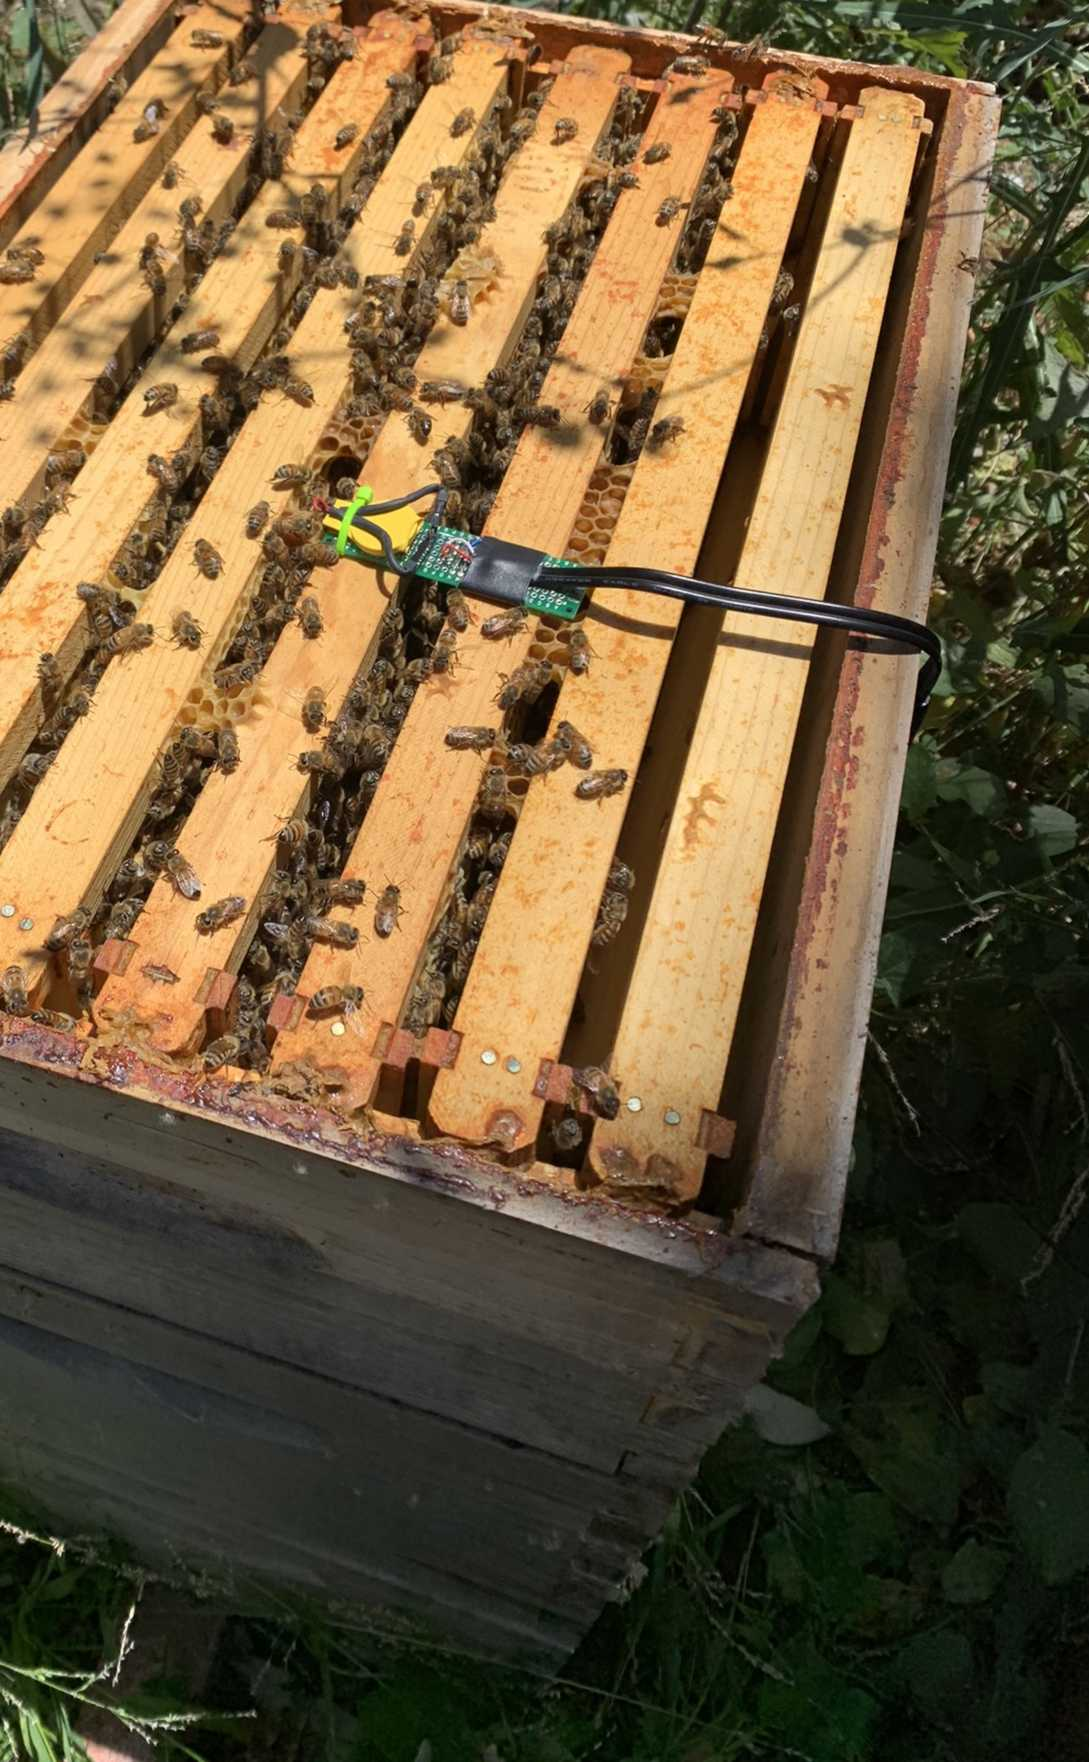
\includegraphics[trim={-10 -20 -10 -10},clip,height=.7\linewidth]{../figs/IMG_4990.jpg}
		}
	\caption{\label{fig::bees}
		a. Sequential zoom into the in-hive communication. 
		Initial agitated state from recently closed hive, can be identified by high amplitude, broad frequency, humming that quiets after about 3000 time slices.
		The bottom zoom window shows that what may look like noisy features in the spectrogram are actually controlled frequency chirps.
		b. Image of a prototype acoustic sensor with frequency response from 20Hz to 85kHz. 
		}
\end{figure}
Figure~\ref{fig::bees} shows the first prototype testing of a tiny ultrasonic microphone, placed inside the beehive, that records the hive humming at well above human acoustic perception.  
The sensors are designed with easily attainable parts, require little advanced knowledge for construction, and cost less than \$3 US each when complete. 
Our team is also providing the AI software and design elements free of charge, to encourage adoption in broader agricultural and environmental-minded communities. 
We also encourage their direct engagement with the community to foster collective solution ownership, and a robust co-design paradigm.

Given the Red Hat origins of the Enterprise Neurosystem community, this project sticks to a philosophy of interdisciplinary open-source sharing of ideas and methods, including hardware integration and software design. 
As a community endeavor, all members share a sense of ownership of the technology.

%\begin{wrapfigure}{l}{.5\linewidth}
%	\centerline{a.}
%	\centerline{
%		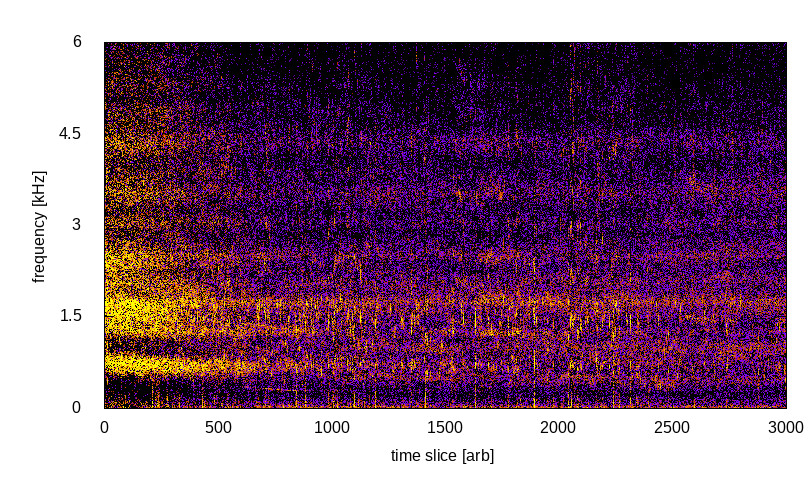
\includegraphics[clip,width=.9\linewidth]{../figs/agitation_filt.jpg}
%		}
%	\centerline{b.\hspace{.3\linewidth}c.\hspace{.3\linewidth}d.}
%	\centerline{
%		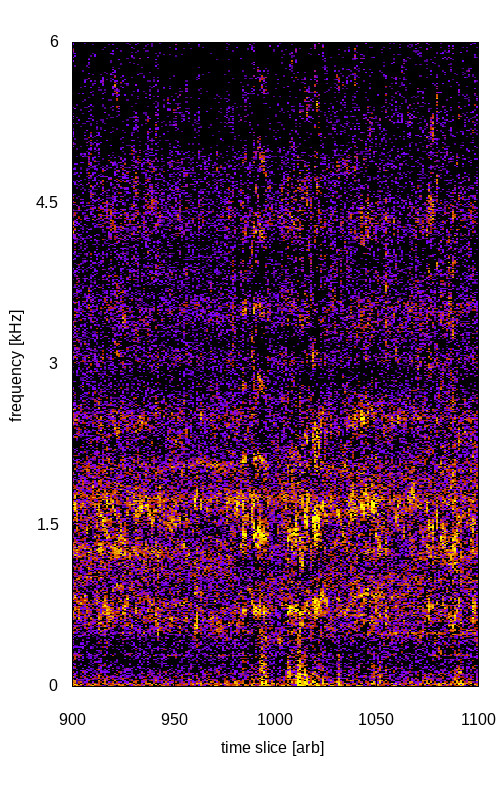
\includegraphics[clip,width=.3\linewidth]{../figs/postagitation_filt.jpg}
%		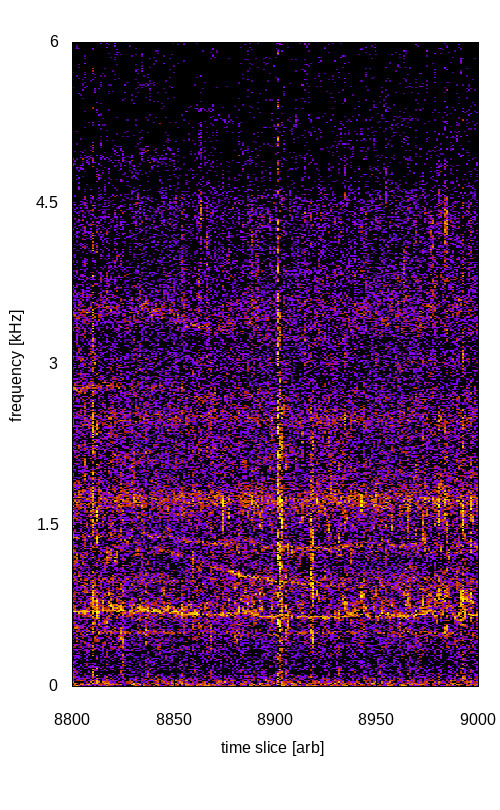
\includegraphics[clip,width=.3\linewidth]{../figs/communicationzoom_filt.jpg}
%		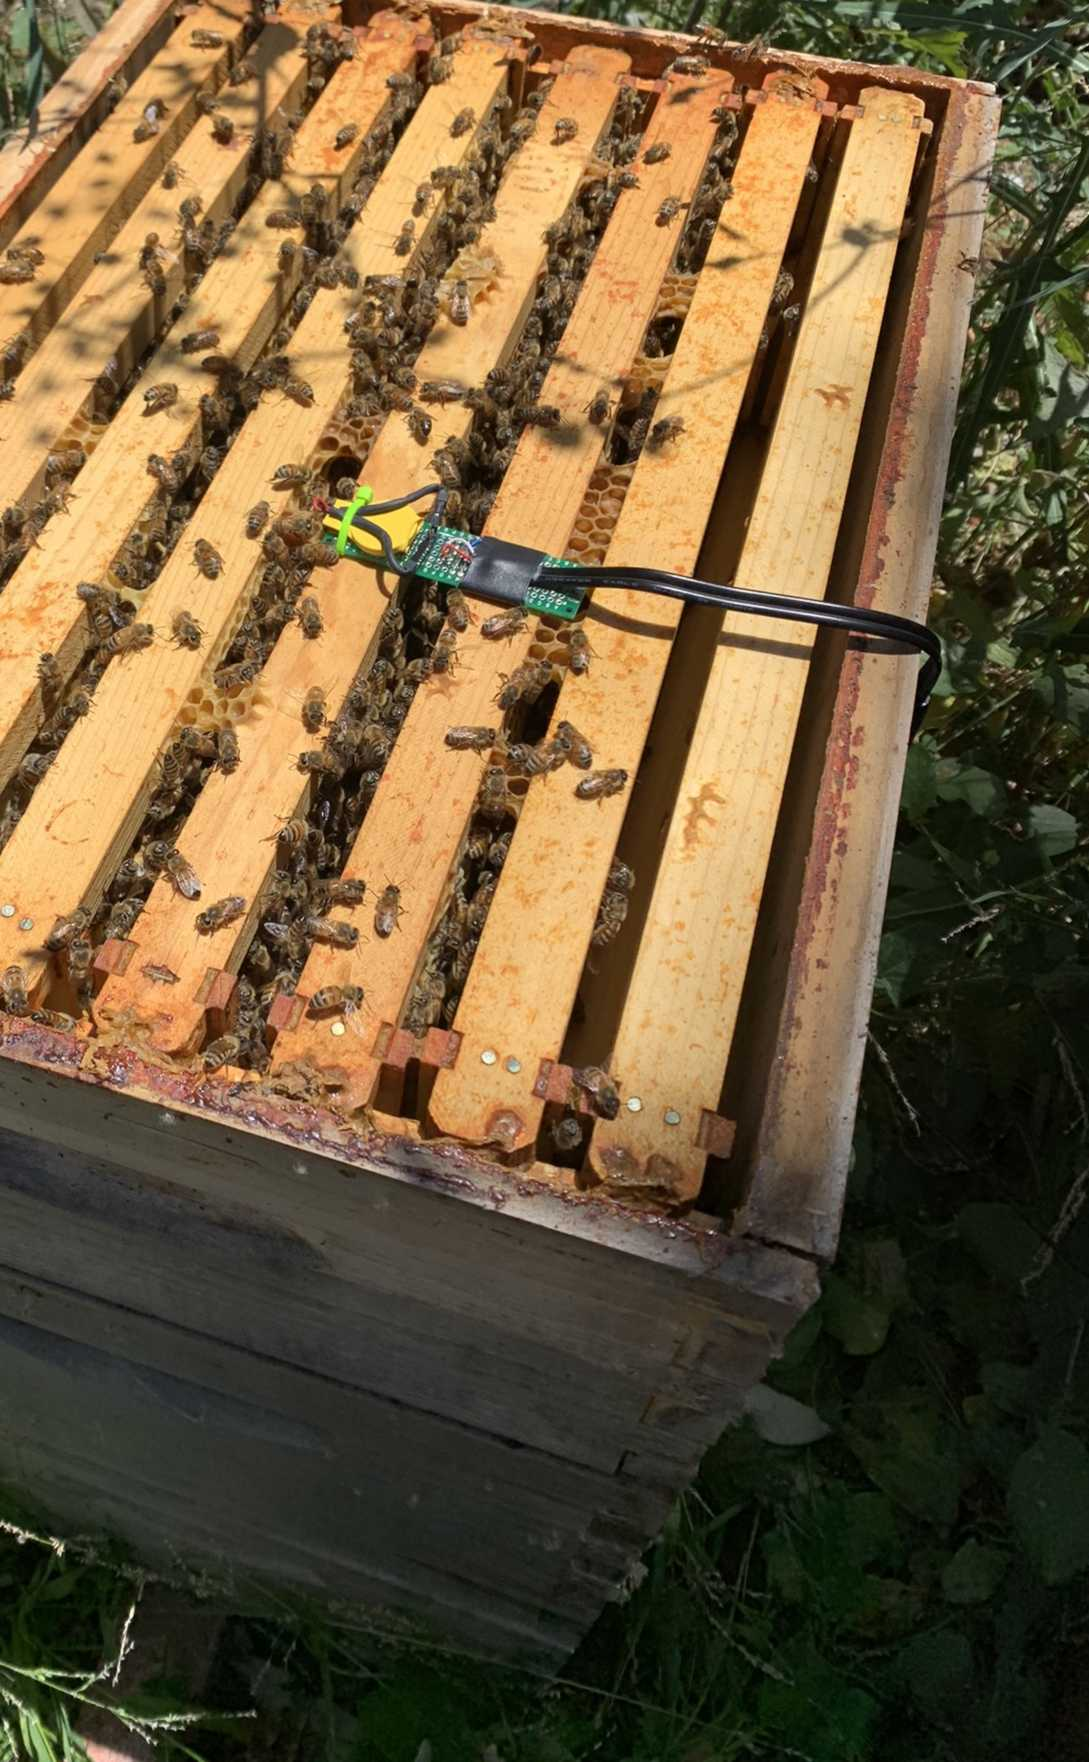
\includegraphics[trim={-25 -50 -25 0},clip,width=.3\linewidth]{../figs/IMG_4990.jpg}
%		}
%	\vspace{-1\baselineskip}
%	\caption{\label{fig::bees}
%		a. Agitated initial state and calming.
%		b. Post-calming communication.
%		c. Calm communication.
%		d. Prototype acoustic sensor with frequency response from 20Hz to 85kHz.
%		}
%\end{wrapfigure}


\paragraph{Sharing is Caring}
As a seed idea to catalyze the direction for this multidisciplinary endeavor for climate and energy resilience, we take inspiration from the accomplishments that so-called Transformer \cite{Attention2017} or Foundation \cite{StanfordFoundationPaper} models have gleaned from tremendously diverse training corpora.
The impressive results in language completion tasks for so-called transformer or foundation models like BERT \cite{bert} and GPT \cite{GPT2018} have been achieved precisely owing to the diverse language corpora available as training sets. 
Unfortunately, the ability of tremendously large models to leverage vast datasets requires equally massive computational capability--a capability typically reserved for major industrial entities and the largest computational facilities in DOE. 


Innovation, however, comes from non-traditional combinations of human ideas, and these combinations shine a spotlight into the gaps between research fields. 
Similarly, large machine learning (ML) models attain “generalizability”' by training across increasingly diverse datasets. 
And although our project is focused on acoustics for hive health, we plan to leverage compatible format data from fields as far-reaching as data-center acoustics and Tokamak magnetic fusion diagnostics (see Fig.~\ref{fig::spectrograms}).

\begin{figure}
	\raggedright{a.}\\
	\centerline{\includegraphics[trim={0 0 0 325},clip,width=\linewidth]{../figs/cerinefigs/ground_truth.png}}
	\raggedright{b.}\\
	\centerline{\includegraphics[trim={0 0 0 325},clip,width=\linewidth]{../figs/cerinefigs/direct_predictions_old_embeddings.png}}
	\caption{\label{fig::spectrograms}
		a. Ground truth spectrogram of ECE signal. b. Forecast of signal by 5ms.}
\end{figure}

\paragraph{Sharing is Daring}
The challenge of open data sharing is a topic that the research sector finds unnervingly challenging. 
The personal motivations that drive researchers to push the limits of possibility are often the same motivations that discourage the open sharing of uniquely produced datasets with understandably competitive community members. 
This personal motivation of Principal Investigators (PIs) is not unlike the intellectual property (IP) concerns of private sector entities, or the economic aspirations of both developed and developing nations.  
As noted in the UN Development Programme's sustainable development goals \cite{SDGs}, addressing global climate goals will require equitable partnerships that respect the economic aspirations of all participants.

The US research ecosystem, in particular across the Department of Energy, represents a functionally similar challenge for equitable data sharing, in support of a cohesive and sustainable future for the broad adoption of AI practices. 
We can only find true success in a multi-modal, data-rich, and geographically and culturally distributed national computing ecosystem. 

Solving a grand challenge and building a far reaching vision, however, always begins with a small exemplar--one hive at a time.



